\section{Results}

The experiment was carried out in Holstebro, Denmark with a diesel Citr\"oen Xantia car. The data collection was done with an iPhone 4s running an app called SensorLog\footnote{http://sensorlog.berndthomas.net/}. The data gathered consisted of GPS, accelerometer. The GPS is sampled at approximately 90 hz.

A total of 22 test runs were driven, three test was not completed due to driver errors, leaving
usable data from 19 test runs. In the processing of data it became apparent that the original way of measuring fuel consumption, by using the meter at the gas pump, and thus were the more reliable measurement method developed (as seen in figure \ref{measured}). Only two test runs were completed with the new method.

\begin{table}
\begin{tabular}{| l | r |}
\hline 
number of trips & 19 \\[0.1cm] \hline
number of datapoints & $12*10^6$\\[0.1cm] \hline
height difference & 6 m\\[0.1cm]
\hline 

\end{tabular}
\label{datatable}
\caption{Description of input data}
\end{table}
map of trip

\begin{figure}[h]
  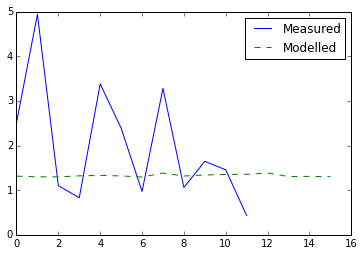
\includegraphics[scale=0.5]{Measured_consumption}
  \caption{The measurement using the pump meter is quite unreliable}
  \label{measured}
\end{figure}

The modelled fuel consumption uses the equation \ref{emission} for each sample point. The speed is the speed estimate gained from the GPS data. Each consumption factor derived from  equation \ref{emission} is the multiplied with the distance from the previous sample point. The distance is calculated from the GPS location and the previous GPS location, using the haversine formula \cite{rick1999deriving} to take the spherical nature of the earth into account.

The modelled fuel consumption from the test has a mean value of 1.32 liters, and a standard deviation of 0.03.

An example speed curve of a run can be seen in figure \ref{speed}.

\begin{figure}[h]
  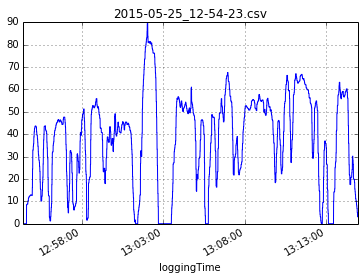
\includegraphics[scale=0.5]{speed}
  \caption{A speed trace for a test run}
  \label{speed}
\end{figure}

The different driving patterns are apparent in the figure, as the large number of speed changes suggests.

\subsection{Acceleration data}

The data from the accelerometer of the smartphone, is used for determine the driving patttern of the driver. Part of the driving pattern is determined by road conditions, such as intersection, stoplights, curves and turning. Other patterns are due to personal driving style, ie. heavy acceleration, overtaking and braking versus more smooth driving, and lastly some patterns are due to traffic conditions, like congested, accidents and slow or fast moving vehicles.
\begin{figure}[h]
  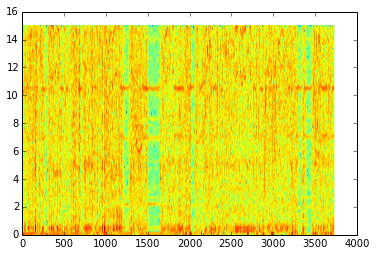
\includegraphics[scale=0.5]{specgram}
  \caption{A spectogram of the magnitude of the acceleration}
  \label{spectogram}
\end{figure}
In figure \ref{spectogram} the magnitude of the acceleration is shown in a spectogram. The x-axis is time (sample number), and the y-axis is the frequency spectrum of the acceleration signal. Form the figure it can be seen that the idle running of the motor, when standing still is very visible, while the motor frequency is not discernible while the vehicle is moving, due to vibrations from the wheels moving on the road.

The spectrogram indicates that the accelerometer signal can be used for detecting an idle running engine in a stationary vehicle.

To be able to discern different driving patterns a simple K-means clustering algorithm was used. There are six driving odes that are of interest: idle, forward acceleration, braking, cruising, left turn, and right turn, thus the number of clusters was chosen to six. Figure \ref{cluster} shows the results of the K-means clustering algorithm on the data from 19 test runs. The clustering is performed separately on each test run, but since the position and orientation of the smartphone was kept the same in all tests (parallel to the vehicle, with X toward the front face (Z) up), we present the results in the same figure. The upper figure shows the X and Y part of the cluster centers, and the two lower figures shows the X, Z part and Y,Z part respectively. There are many cluster centers close the the origin of the graph, corresponding to either idle or cruising driving mode. Many of the test have two centers at or close to the origin in the X,Y chart, indicating that the Z axis differs in the two cases, which is expected from the difference between idle (no road vibration) and cruising (road vibration).

The X,Z and Y,Z charts of the cluster centers are aligned along $X=0$ and $Y=0$ axis, again indicating that the Z value of centers are connected to low acceleration i X or Y.
\begin{figure}[h]
  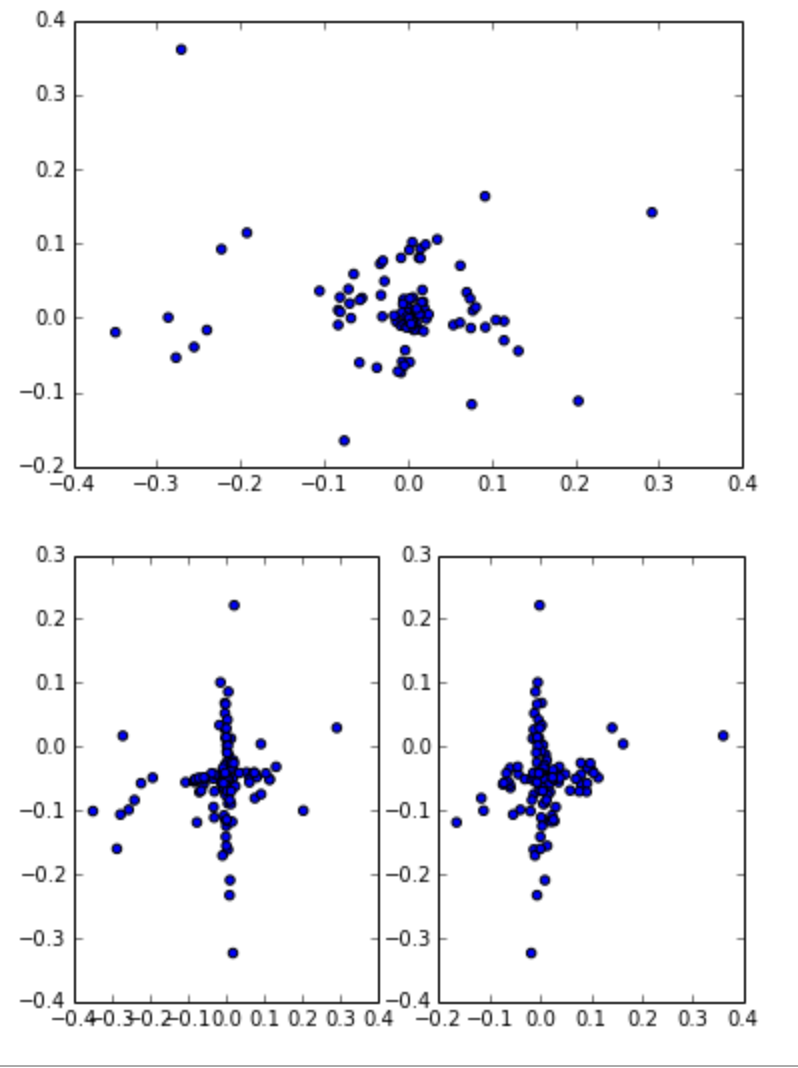
\includegraphics[scale=0.5]{cluster_acc}
  \caption{Clustering of accelerometer data}
  \label{cluster}
\end{figure}

To further improve the detection of the driving mode, a low pass filter was applied to the three different acceleration signals, before performing the K-means clustering. The result for the X,Y plane is shown in figure \ref{cluster2}
\begin{figure}[h]
  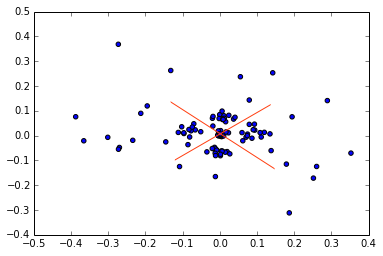
\includegraphics[scale=0.5]{cluster_acc2}
  \caption{Clustering of low-pass filtered accelerometer data}
  \label{cluster2}
\end{figure}

With the added low pass filter, a good separation between the driving modes, is apparent. the added lines indicate how to discern between the the four accelerating modes: forward, brake, left turn, and right turn. To discern between idle and cruising one have to take the Z axis signal into account as well, or consider the speed signal from the GPS.  

